% -----------------------------------------------
% Template for ISMIR Papers
% 2015 version, based on previous ISMIR templates
% -----------------------------------------------

\documentclass{article}
\usepackage{ismir,amsmath,cite}
\usepackage{graphicx}
\usepackage{color}
\usepackage{amsfonts}
\usepackage{brian}
\usepackage{qtree}
\usepackage{caption}
\usepackage{subcaption}
% \def\shag{\ensuremath{\text{\textsc{SHAG}}}}
%\def\shag{\ensuremath{\mathpzc{H}}}
\def\shag{\ensuremath{\mathpzc{T}}}
\DeclareMathAlphabet{\mathpzc}{OT1}{pzc}{m}{it}

% Title.
% ------
\title{Hierarchical Evaluation of Music Segment Boundary Detection}

% Single address
% To use with only one author or several with the same address
% ---------------
%\oneauthor
% {Names should be omitted for double-blind reviewing}
% {Affiliations should be omitted for double-blind reviewing}

% Two addresses
% --------------
\twoauthors
  {First author} {School \\ Department}
  {Second author} {Company \\ Address}

% Three addresses
% --------------
%\threeauthors
  %{First author} {Affiliation1 \\ {\tt author1@ismir.edu}}
  %{Second author} {\bf Retain these fake authors in\\\bf submission to preserve the formatting}
  %{Third author} {Affiliation3 \\ {\tt author3@ismir.edu}}

% Four addresses
% --------------
%\fourauthors
%  {First author} {Affiliation1 \\ {\tt author1@ismir.edu}}
%  {Second author}{Affiliation2 \\ {\tt author2@ismir.edu}}
%  {Third author} {Affiliation3 \\ {\tt author3@ismir.edu}}
%  {Fourth author} {Affiliation4 \\ {\tt author4@ismir.edu}}

\begin{document}
%
\maketitle
%
\begin{abstract}
Structure in music is traditionally analyzed hierarchically: large-scale sections at the highest level can be sub-divided and refined down to the short melodic ideas at the motivic level. 
However, typical algorithmic approaches to structural annotation produce flat temporal partitions of a track, which are commonly evaluated against a similarly flat, human-produced
annotation. This effectively discards all notions of structural depth in the evaluation.
Recently, collections of hierarchical structure annotations have been published, but at present, no evaluation techniques exist to evaluate against these rich structural annotations.
We propose a method to evaluate structural boundary detection in the context of hierarchical annotation.
The proposed method transforms boundary detection into a ranking problem, and facilitates the comparison of flat and hierarchical annotations.
We demonstrate the proposed method with various synthetic and real examples. 
\end{abstract}
%
\section{Introduction}\label{sec:introduction}

The analysis of the structure in music has been one of the main areas of interest by musicologists for many years.
Its goal is to identify and categorize the form of a musical piece by investigating the organization of its components, such as sections, phrases, melodies, or recurring motives.
Traditional analyses usually provide multiple levels of annotation (\eg, Schenkerian analysis), which reinforce the general assumption that music is structured hierarchically~\cite{Lerdahl1983a}.
Consequently, tree representations are commonly used to both model and analyze hierarchical forms in music~\cite{Lerdahl1983}.

In the music information research literature, \emph{music segmentation} (also known as \emph{music structure analysis}) is a task that aims to automatically identify the structure of music~\cite{Paulus2010}.
Historically, the segmentation task has been geared toward the design of algorithms which partition a song into non-overlapping (or \emph{flat}) segments of time.
Nevertheless, it has been shown that even these segments tend to be organized in a hierarchical manner~\cite{Peeters2009}, and even a large dataset of hierarchically-structured human annotations is now publicly available~\cite{Smith2011}.
% Still, most existing algorithms only operate at a flat level, likely because (i) this task is already challenging at this level~\cite{Skywalker2014}, and (ii) even if an algorithm could 
% estimate hierarchical segments, no method to evaluate them has been proposed.
However, current evaluation methodologies are defined only for flat segmentations, both in the estimation (algorithm output) and reference human annotation data.
Therefore, the dimension of \emph{depth} has been practically ignored in the evaluation of music segmentation algorithms.
This contrasts with the task of \emph{pattern discovery}, where overlapping segments that do not necessarily cover the entire piece are allowed, and numerous metrics to evaluate these patterns have been proposed~\cite{Collins2013}.
These two tasks share multiple attributes~\cite{Nieto2014_Motives}, and steps toward a more general formulation musical structure analysis could be made by evaluating segmentation in 
a hierarchical manner.

%This automatic task could facilitate, e.g., the intra-piece navigation, generation of music summaries, or segment-based recommendation systems, especially nowadays when listeners have easy access to large digital music collections.
%Nevertheless, the vast majority of music segmentation algorithms only operate at a flat level instead of following the hierarchical approach that most musicologists follow.

\subsection{Our contributions}
In this work we present the \emph{Tree Measures} ($T$-measures), a set of scores to evaluate the accuracy of boundary detection in hierarchical segmentations.
%The proposed metrics work at a frame-level --- similar to the method proposed by Levy and Sandler to evaluate structural annotations~\cite{Levy2008} --- and they are based on a rank retrieval evaluation where each frame is ranked depending on whether it belongs to the \emph{correct} segment.
In simple terms, the proposed $T$-measures operate by first computing similarities between frames of a track according to distance in the hierarchy, and these similarities are scored by
a measure of ranking correlation against the reference annotation.
The segmentation is evaluated simultaneously across all hierarchical layers, and the resulting scores can be applied to either hierarchical or flat boundary annotations.
%(Note that a flat segmentation is only a specific case of a hierarchical one, where the number of layers is one.)
With the $T$-measures, we facilitate the evaluation of existing flat estimations against hierarchical reference annotations (like those of~\cite{Smith2011}), and encourage new publications on richer hierarchical algorithms.
We demonstrate the behavior of the $T$-measures with multiple synthetic and human examples, and compare the scores with the existing methods when possible.

%The rest of the paper is organized as follows:
%In \cref{sec:curr_meth} we review the current evaluation methods of (flat) boundary algorithms. 
%The proposed metric is formally introduced in \cref{sec:eval_desc}. 
%We provide multiple examples to illustrate the behavior of the $T$-measures in \cref{sec:examples}.
%Finally, we draw conclusions and discuss future work in \cref{sec:conclusions}.

\section{Segment Boundary Evaluation}\label{sec:curr_meth}

Music segmentation algorithms are typically evaluated for two distinct goals.  
The first goal, known as \emph{boundary detection}, evaluates the estimated segmentation's accuracy at detecting the times of transitions between segments.
The second goal, known as \emph{structural annotation}, evaluates the labeling applied to the estimated segmentation, and thus quantifies the ability of an
algorithm to detect repeated forms, such as verses or refrains. 
In this paper, we focus exclusively on the boundary detection task.

Boundary estimates are primarily evaluated in terms of precision and recall~\cite{turnbull2007supervised}.
Formally, estimated and reference boundaries are matched within a specified tolerance window ---typically either 0.5 or 3 seconds--- and the hit rate $n_h$ (number of successful matches) is used to define precision and recall scores:
\begin{equation}
P \defeq \frac{n_h}{n_e}, \quad\quad R \defeq \frac{n_h}{n_r},
\end{equation}
where $n_e$ and $n_r$ denote the number of boundaries in the estimated and reference
annotations, respectively.
As is standard in information retrieval, $P$ and $R$ are combined into an $F$-measure by computing their harmonic mean.

Boundary estimation has also been evaluated by \emph{deviation}~\cite{turnbull2007supervised}.
This is done by measuring the median time (absolute) differential between each reference boundary and the nearest estimated boundary (\emph{R2E}), and vice versa (\emph{E2R}).
Boundary deviation is useful for quantifying the temporal accuracy of a detection event.
However, it can be sensitive to the number of estimated boundaries.

\subsection{The limitations of flat evaluation}
The precision-recall paradigm has been critical to quantifying improvements in segmentation algorithms over the past several years, but it has obvious limitations.
First, it confines both the reference and estimated annotations to have a flat structure.
This is sometimes resolved by collecting multiple flat annotations for each track, each corresponding to a different level of analysis~\cite{Smith2011}.  

When evaluating a segmentation algorithm, it is not immediately clear how one should report accuracy when evaluating multiple layers for each track.
For example, direct aggregation of accuracy scores across layers would imply that boundaries at all layers are equally important.
Moreover, due to hierarchical constraints, boundaries at low levels outnumber those at high levels, which may convey more information about the overall structure of the piece, but end up contributing less to the overall metric.

On the other hand, reporting statistical score summaries for each individual layer can be problematic as well.
If the dataset is heterogeneous and spans many genres, there may be no consistent way in which to stratify hierarchical levels across the entire collection.
The resulting scores may exhibit unnecessarily high variance due simply to ill-defined stratification parameters.

Furthermore, by evaluating each level independently, the relational structure between layers is lost.
As an example, \cref{trees} depicts two distinct structural decompositions of a song $S$, first into high-level components $A$ and $B$, and then into small components $a, b, c$.
While both trees produce the same set of boundaries at each level, the structural interpretation is significantly different.
This hierarchical information would be lost by any form of independent, layer-wise evaluation.

\begin{figure}
\Tree[.S [.A [.\emph{a} ] [.\emph{b} ] ] [.B \emph{c} ] ]
\Tree[.S [.A [.\emph{a} ] ] [.B [.\emph{b} ] [.\emph{c} ] ] ]
\caption{A toy example of two hierarchical annotation structures with identical flat segmentations at each layer ---$(A, B)$ and $(a,b,c)$---  but distinct structural interpretations.\label{trees}}
\end{figure}

\section{The Tree Measures}\label{sec:eval_desc}
\sloppy
In this section, we derive the \emph{tree measures} for evaluating multi-level structural boundary detection.
%The proposed evaluation scheme explicitly accounts for cross-layer structure in segmentation, and directly accommodates multiple layers of specificity in both the reference and estimation.
The evaluation is based on a reduction to ranking evaluation, which we describe in detail below.

\subsection{Preliminaries}

% Let denote a song as represented by a time series of 
% feature data, where $d$ denotes the dimension of features, and $n$ denotes the
% time duration at some fixed resolution $f_r$ (\eg, 10Hz).
% Flat segmentation evaluation schemes suppose a single partitioning into $m$
% temporally contiguous regions, so that $X=[X_1|X_2|\cdots|X_m]$.  
% Instead, we will allow for a hierarchical decomposition

Let $S $ denote a flat, temporally contiguous partition of the time range spanning the track in question.
We will use the subscripts $S_R$ and $S_E$ to denote \emph{reference} and \emph{estimation}, respectively.
We will assume that samples are generated at some fixed resolution $f_r$ (\eg, 10Hz), although non-uniform samplings (\eg, beat- or onset-aligned samples) are easily accommodated.  
$S(i)$ will denote the identifier of the partition containing the $i$th sample.
As in frame-based structural annotation evaluation, we require that the same collection of samples be applied to both reference and estimated annotations~\cite{levy2008structural}.

Hierarchical segmentations will be denoted by $H_R$ and $H_E$ for reference and estimated annotations.
For a hierarchical segmentation $H$, $H(i,j)$ will denote the most specific segment containing samples $i$ and $j$.
We will denote precedence (containment) of segments by $\prec$: \eg, $H(j, k) \prec H(i, k)$.

To exemplify this notation, a three-level hierarchy is plotted in \Cref{fig:hier-example}.
In this context, $H(i, i)$ denotes the most specific segment containing frame $i$, which is the first segment in ``level\_2.''
Similarly, $H(j,j)$ and $H(k,k)$ refer to the second and third segments in  ``level\_2``, while $H(j,k)$ refers to their least common ancestor: the second segment in ``level\_1``.
We can then infer membership and precedence relations, such as
\begin{equation}
j \in H(j, j) \prec H(j, k) \prec H(i, j) = H(j, k).
\end{equation}


\begin{figure}
  \centering
  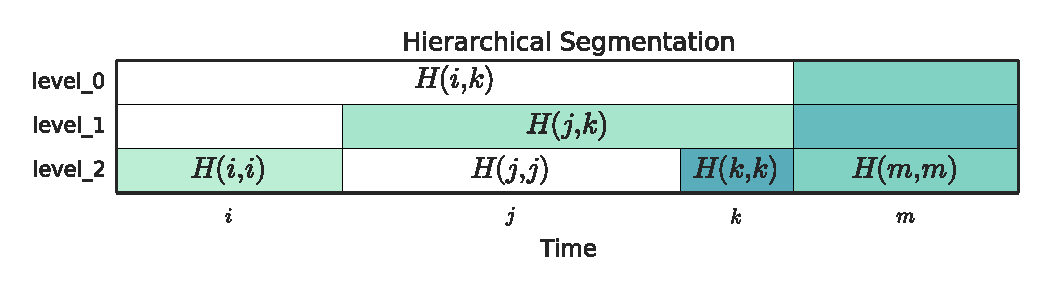
\includegraphics[width=0.45\textwidth]{figs/hier-example.pdf}
  \caption{An example of a synthetic, three-level hierarchical segmentation.
  Frames $i, j, k,$ and $m$ are indicated along the $x$-axis, and some of their containing segments are indicated within the figure, \eg, $H(i, j)$.}
  \label{fig:hier-example}
\end{figure}

Note that flat segmentations are a special case of hierarchical segmentations, where there is one node at the root of the hierarchy containing all samples, and then $m$ segments at the next level down which form a full partition of the track.

If we restrict attention to a query sample $q$, then $H(q, \cdot)$ induces a partial ranking over the remaining samples.
Frames contained in $H(q, q)$ are considered maximally relevant, followed by those in $H(q, \cdot)$'s immediate ancestor, and so on.
This observation will be the key to our evaluation, as it provides a connection between hierarchical time-series decompositions and ranking evaluation.

\subsection{Flat segmentation and bipartite ranking}

We can reduce segmentation evaluation to a ranking evaluation problem as follows.
Let $q$ denote an arbitrary frame, and let $i$ and $j$ denote any two frames such that $S_R(q) = S_R(i)$ and $S_R(q) \neq S_R(j)$.
In this case, $i$ may be considered \emph{relevant} for $q$, and $j$ is considered \emph{irrelevant} for $q$.
This leads to a straightforward reduction to bipartite ranking.

A per-frame recall metric can be formally defined as
\begin{equation}
f(q ; S_E) \defeq 
\sum_{\substack{i \in S_R(q)\\ j \notin S_R(q)}}
\frac{\ind{S_E(q) = S_E(i) \neq S_E(j) }}{|S_R(q)|\cdot (n -
|S_R(q)|)}.\label{flatrecall}
\end{equation}
where $\ind{\cdot}$ is the indicator function, and $n$ denotes the number of frames in the track.
The score for frame $q$ is the fraction of pairs $(i, j)$ for which $S_E$
agrees with $S_R$ with respect to $q$ (\ie, membership in the segment).

Averaging over all frames $q$ yields a mean sample recall score:
\begin{equation}
\rho(S_E) \defeq \frac{1}{n} \sum_q f(q ; S_E).\label{avgrecall}
\end{equation}
% TODO:   2014-05-05 00:38:15 by Brian McFee <brm2132@columbia.edu>
% talk about why we don't need to consider precision here
% predictions are mutually exclusive
% the usual way to cheat at recall is to make too many predictions..
% but to do that for q1, you'd have to make fewer predictions for q2,
\nocite{levy2008structural}


\subsection{Hierarchies and partial ranking}

\Cref{flatrecall} is defined in terms of segment membership (in)equalities, but we can equivalently express the function using strict precedences in a (flat) segment hierarchy.
Rather than compare $i$ and $j$ where $S(q) = S(i) \neq S(j)$, we can express this as $H(q, i) \prec H(q, j)$.
That is, the pair $(q,i)$ merge deeper in the hierarchy than do $(q,j)$:
\begin{equation}
g(q ; H_E) \defeq \sum_{\substack{(i, j)\\ H_R(q, i) \prec H_R(q, j)}}
\frac{\ind{H_E(q, i) \prec H_E(q, j)}}{Z_q},\label{hierrecall}
\end{equation}
where $Z_q$ is a normalization term that counts the number of terms in the summation.

Just as in \cref{flatrecall}, $g$ can be viewed as a classification accuracy of correctly predicting pairs $(i, j)$ as positive ($q$ and $i$ merge first) or negative ($q$ and $j$ merge first).
The case where $H(q, i) = H(q, j)$ is precluded by the strict precedence operator in the summation.

\Cref{hierrecall} can be alternately be viewed as a generalized area under the curve (AUC) over the partial ranking induced by the hierarchical segmentation, where depth within the estimated hierarchy $H_E$ plays the role of the relevance threshold.

Because $g(q; H_E)$ acts as a generalization of recall, an estimate $H_E$ will achieve a low score if it fails to distinguish between pairs $i$ and $j$.
Similar to the normalized conditional entropy metrics for structural estimation, this can be interpreted as a form of \emph{under-segmentation}, in that a low score indicates either an ordering error or a lack of specificity~\cite{Lukashevich2008}.  

% Note that the precedence comparisons here are strict, so we never compare two $i$ and $j$ that merge simultaneously with $q$.
By aggregating over all sample frames $q$, we obtain the \emph{under-segmentation} $T$-measure:
\begin{equation}
\shag_u(H_E) \defeq \frac{1}{n} \sum_q g(q ; H_E).\label{shagunder}
\end{equation}
The over-segmentation metric $\shag_o(H_E)$ is defined analogously by swapping the roles of $H_E$ and $H_R$ in \cref{hierrecall}.
Combined, the two metrics summarize structural agreement between estimated and reference hierarchical annotations.

% Note this loss is equivalent to that evaluated by for subjective artist similarity~\cite{mcfee2011}.
% The difference here is that the reference rankings are induced from ordinal data, and not subject to consistency errors.

\subsection{Windowing in Time}

The $T$-measures above capture the basic notion of hierarchically nested, frame-level relevance, but they pose two technical limitations.
First, the score for each query will generally depend on the track duration $n$, which makes comparisons between tracks of differing length problematic.  
For large values of $n$, \cref{hierrecall} may be dominated by trivially irrelevant comparison points $j$ which lie far from $q$ in time, \ie, $|q-i| \ll |q-j|$.
Short-duration tracks with small $n$ have fewer such trivial comparisons.
Therefore, longer tracks may observe relatively inflated scores when compared to shorter tracks, simply by virtue of having a large number of ``easy'' comparisons.
Moreover, the calculation of the $T$-measures as defined in \cref{shagunder} can be expensive, taking $\Oh(n^3)$ using a direct implementation.

To resolve these issues, we propose to use a time window of $w$ seconds in order to both simplify the 
calculation of the metric and normalize its dynamic range.
We restrict the number of samples under consideration to $m = \lceil w \cdot f_r \rceil$.
Adding this windowing property to equations (\ref{hierrecall},~\ref{shagunder}) yields the windowed $T$-measures:
\begin{equation}
  g(q, m ; H_E) \defeq \sum_{\substack{
  m_s \leq i,j \leq m_e \\ 
  H_R(q, i) \prec H_R(q, j) }} \frac{\ind{H_E(q, i) \prec H_E(q,
  j)}}{Z_q(m)},\label{windowrecall}
\end{equation}
\begin{equation}
\shag_u(H_E, m) \defeq \frac{1}{n} \sum_q g(q,m ; S_E),
\end{equation}
where $m_s = \min\{0,q-m/2\}$ and $m_e = \max\{q+m/2,n\}$ are the start and ending, respectively, of the current window in sample indices.
The resulting metric has reduced computational complexity $\Oh(nm^2)$.  Moreover, excluding edge cases near the beginning and end of the track, each query frame $q$ now operates over a
fixed number of comparisons $(i, j)$, regardless of the track duration.

\subsection{Choosing a time window}

The choice of window size will clearly have a dramatic impact on the evaluation.
Small windows (\eg, $w \leq 3$) generally capture local changes, since large-scale structural changes are not typically confined to such small time intervals~\cite{Smith2013}.
Ideally, the window should be long enough to capture boundaries of segments at multiple resolutions, but not so large as to become dominated by trivial comparisons.
While there may not be a single window length that satisfies this criteria for all songs, we consider two practical approaches to window selection.

First, an appropriate window length can be estimated by examining the segment duration statistics of the reference annotations.  
For example, one may take the average duration of high-level segment annotations, as they can be expected to contain multiple small segments, and thus capture local structure.
Second, one may report results for a multiple window parameters, as is currently done for boundary detection as described in \cref{sec:curr_meth}.  

% Ideally, the window should be long enough to capture the boundaries of the current segments, and that is the same for all tracks in order to be able to easily compare results within a reasonable dynamic range.


\subsection{Transitive reduction}

Just as \cref{hierrecall} can be dominated by long-range interactions in the absence of windowing, deep hierarchies can also pose a problem.
To see this, consider the sequence $H_R(q, i) \prec H_R(q, j) \prec H_R(q, k)$.
Due to the transitive containment structure of $H_R$, we have $i \in H_R(q, i) \subseteq H_R(q, j)$.
Since the summation in \cref{hierrecall} ranges over all precedence comparisons, the pair $(i, k)$ appears twice in the summation when computing the
recall from frame $q$.  Since segments grow in size at higher levels in the hierarchy, this over-counting can dominate the score function as well.

To counteract this effect, the summation can be restricted to only range over direct precedence relations.
In practice, this is accomplished by only comparing samples from successive levels in the hierarchy, \ie, 
replacing the partial ranking generated by $q$ with its transitive reduction.
This eliminates redundant comparisons and increases $g$'s dynamic range.


\section{Examples}\label{sec:examples}

In this section we discuss the behavior of the $T$-measures by showing various synthetic examples, and compare them against other existing methods when possible.
%We show the two grades of $T$-measures (undersegmentation, oversegmentation) for all the examples in this sections
%Two different versions of each metric are used to evaluate these examples: Estimated against Reference boundaries (E2R), and the Reference boundaries against the Estimated ones (R2E).
%These results will help us illustrate the variation of the scores when swapping the references with the estimations, which, in the case of $T$-measures, has a significant impact.
For each example in this section, we illustrate the behavior of our proposed metric under different window times $w$.
This section is subdivided by type of annotations under consideration.

\subsection{Flat vs Flat}

To start with, we compare two flat boundary annotations (\ie, one-layer), and see how the $T$-measures behave compared to the standard hit rate measure at 3 seconds, as well as boundary deviation scores.
The synthesized flat boundaries are displayed on the top of \Cref{fig:flat-flat}, and they aim to capture a situation where an algorithm only estimates ---without any time deviations--- a subset of all the reference boundaries.

Since we are evaluating flat annotations, we can compute the standard metrics as well.
The hit rate scores (top right part of the table of \Cref{fig:flat-flat}) obtain a precision of 100\%, since all the estimated boundaries are also in the reference.\footnote{For boundary detection metrics, we trim the first and last boundaries, as they mark the beginning and of the track, and are constant across all estimates.}
On the other hand, only four out of seven boundaries were retrieved, so the recall value is 40\%, leaving the F-measure at 57.14\%.

The median deviations, displayed on the bottom right of the table, are always 0 seconds ---the best possible score--- both when evaluating the Estimation against the Reference (E2R) and vice versa (R2E), since we did not add any fluctuation in the boundaries.
It becomes apparent how boundary deviation metrics are not always reliable, since two sets of boundaries can be quite structurally different while still obtaining the best results for this metric.

\begin{figure}
  \centering
  \begin{subfigure}{0.5\textwidth}
    \centering
    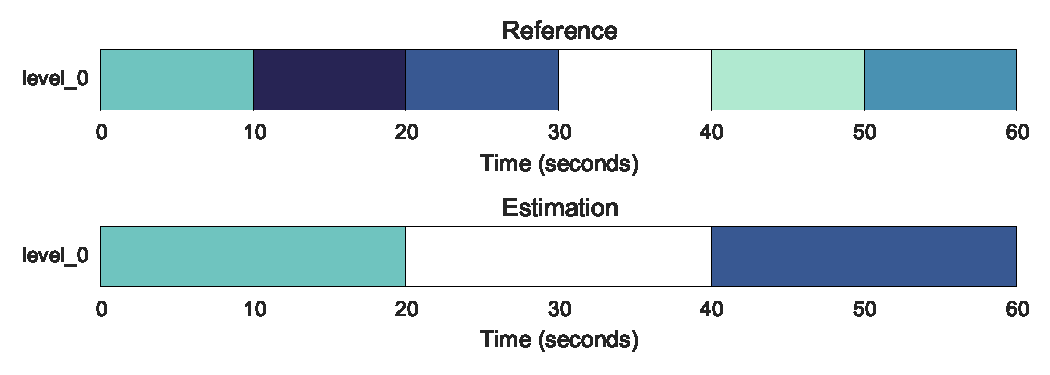
\includegraphics[width=0.94\textwidth]{figs/flat-flat.pdf}
  \end{subfigure}%
  \\
  \begin{minipage}{0.5\textwidth}
    \centering
    \vspace{10pt}
    \begin{tabular}{|c|c|c||c|c|c|}
      \hline
      \multicolumn{3}{|c||}{\textbf{$T$-measures}} & \multicolumn{3}{c|}{\textbf{Hit Rate (trimmed)}} \\
      \hline
      $w$ & $\shag_u$   & $\shag_o$ & $F$     & $P$     & $R$ \\
      \hline
      0.5       & 40.0   & 100   & 57.14  & 100 & 40.0 \\
      \cline{4-6}
      3         & 40.0   & 100  \\
      \cline{4-6}
      15        & 39.39  & 52.77 & \multicolumn{3}{c|}{\textbf{Median Deviations}}   \\
      \cline{4-6}
      30        & 69.46  & 49.75 & \multicolumn{2}{c|}{E2R} & 0 \\
      $\infty$  & 80.0   & 49.75 & \multicolumn{2}{c|}{R2E} & 0 \\  
      \hline
    \end{tabular}
  \end{minipage}
  \caption{Flat vs.\ flat boundaries (top), $T$-measures and boundary hit-rate
  scores (bottom).  In the boundary plots, black indicates segment membership agreement, and white indicates disagreement.}
  \label{fig:flat-flat}
\end{figure}

The $T$-measures for the flat annotations are shown on the left side of the table in \Cref{fig:flat-flat}.
% Since the estimated boundaries are under-segmented, we obtain a low score for $\shag_u$. The estimation does not over-segment at any point, and achieves a perfect score on $\shag_o$.
% In this case, $T$-measures scores match precision and recall values at short time windows. This is because we are only evaluating one level of boundaries, and $P$ and $R$
% also capture the amount of under and over-segmentation of the estimation respectively.
When the windows are smaller than the segments, the $T$-measures behave as boundary detection metrics.
This is evidenced by the $\shag_u$ and $\shag_o$ matching recall and precision for $w \leq 3$.
For the longer time windows, we observe that $\shag_o$ decreases, while $\shag_u$ increases.
To understand this, consider the following examples.
First, let $(q,i,j) = (5,15,25)$.
In this case, the estimation considers $i$ to be relevant for $q$ (since they belong to the same large segment), and $j$ to be irrelevant for $q$; meanwhile, the reference considers both $i$ and $j$ to be equally irrelevant for $q$.
Note that this type of comparison only enters the evaluation for sufficiently large windows, at which point, the over-segmentation score decreases.  

In the other direction, $(q,i,j) = (5, 7, 15)$ causes similar behavior in the under-segmentation metric.
As $w$ increases, the evaluation becomes dominated by long-range interactions, and these localized discrepancies matter less.
As a result, the under-segmentation metric increases when $w$ becomes sufficiently large.
This illustrates how the window size must depend on the duration and scale of structure that the practitioner wishes to capture. 

\subsection{Flat vs hierarchical}

Here we present two different examples of flat estimations (large- and small-scale) against a hierarchical reference.
This situation often arises when we try to evaluate an algorithm that tends to under-segment (large scale) or over-segment (small scale) against a track that is annotated
hierarchically, such as in the SALAMI dataset.

\subsubsection{Flat, large-scale}

In this example, we show the behavior of $T$-measures when comparing a large-scale flat estimation against a hierarchical reference.
On the top of \Cref{fig:hier-flatlarge}, the boundaries are plotted.
The estimated boundaries in this example correspond to the highest layer of the hierarchical reference annotation.
At the bottom of this figure, we observe that $T$-measures behave as expected: the over-segmentation value $\shag_o$ is always 100\%, since the reference annotation agrees with the estimation at the high level.
When using small time windows ($w \leq 3$), the under-segmentation score is 40\%, also as expected, since it resembles the situation of the first example, but adding an extra layer in the reference.
%However, as $w$ increases, the $T$-measures calculation captures multiple levels of granularity, and the metric is able to correctly rank the flat boundaries against the hierarchical ones.
%As a result, the under-segmentation score increases at larger $w$, indicating the importance of choosing a sufficiently large window.


\begin{figure}
  \centering
  \begin{subfigure}{0.5\textwidth}
    \centering
    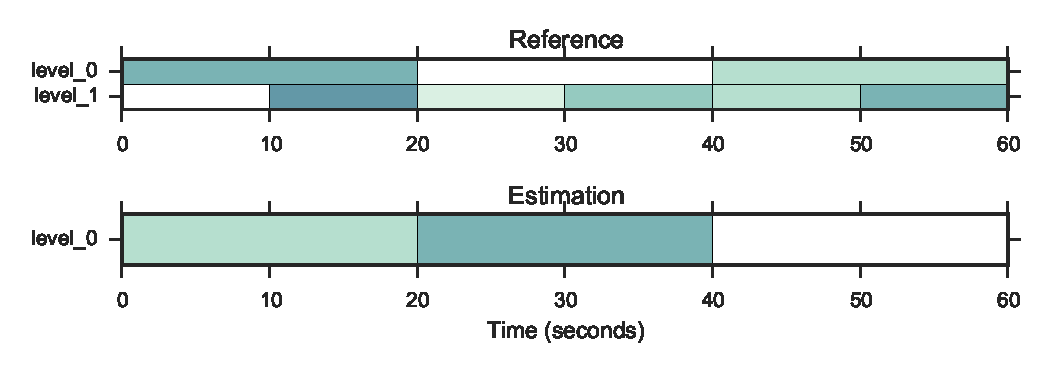
\includegraphics[width=0.94\textwidth]{figs/hier-flatlarge.pdf}
  \end{subfigure}%
  \\
  \begin{minipage}{0.5\textwidth}
    \centering
    \vspace{10pt}
    \begin{tabular}{|c|c|c|}
      \hline
      $w$       & $\shag_u$    & $\shag_o$      \\
      \hline
      0.5       & 40.0      & 100      \\     
      3         & 40.0      & 100      \\
      15        & 51.01     & 100    \\
      30        & 81.76     & 100    \\
      $\infty$  & 88.94     & 100    \\
      \hline
    \end{tabular}
  \end{minipage}
  \caption{Hierarchical reference vs.\ flat (large-scale) estimation (top) and $T$-measures (bottom).}
  \label{fig:hier-flatlarge}
\end{figure}

\subsubsection{Flat, small-scale}

Here we analyze the behavior of $T$-measures in the case of a flat algorithm that tends to over-segment its estimations, producing small-scale estimated segments.
The boundaries and resulting scores are found on the top and bottom of \Cref{fig:hier-flatsmall}.
% Since, as in the large scale case, we are not over-segmenting, the over-segmentation grades are 100\% for all the time windows.
As in the previous example, the hierarchical reference contains boundaries at the same level of granularity as the estimation. 
Because the reference and estimate agree at the lowest level, the over-segmentation score is maximal for all time windows.
% As opposed to the previous example, now the lower layer of the reference boundaries match exactly with the estimations, that results into perfect under-segmentation scores for the shorter time windows.
% In this case, the higher the $w$, the lower these under-segmentation grades as expected, since we should not evaluate an algorithm as perfect if it only identifies one layer of the hierarchical boundaries found in the reference.
Note, however, that the reference provides strictly more information than the estimate.  For example, the estimate considers samples at $t=15$ and $t=45$ to be equally irrelevant for a 
query at $t=5$, while the reference indicates a preference for $t=15$.  These effects are only apparent for sufficiently large window sizes, \eg, larger than the smallest level of
detail, which in this case, is 15s.  This can be easily observed in the $\shag_u$
scores in \Cref{fig:hier-flatsmall}, which drop rapidly once the window size becomes
large enough to span multiple small segments.

\begin{figure}[t]
  \centering
  \begin{subfigure}{0.5\textwidth}
    \centering
    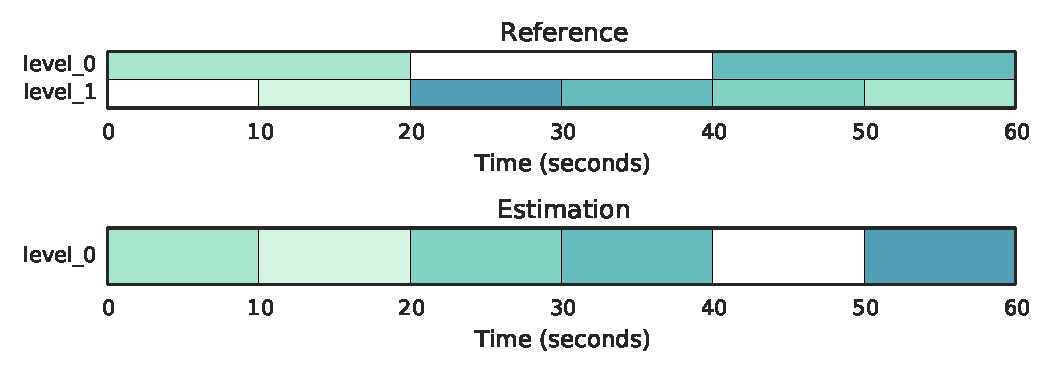
\includegraphics[width=0.94\textwidth]{figs/hier-flatsmall.pdf}
  \end{subfigure}%
  \\
  \begin{minipage}{0.5\textwidth}
    \centering
    \vspace{10pt}
    \begin{tabular}{|c|c|c|}
      \hline
      $w$       & $\shag_u$    & $\shag_o$      \\
      \hline
      0.5       & 100       & 100      \\     
      3         & 100       & 100      \\
      15        & 76.31     & 100    \\
      30        & 58.91     & 100    \\
      $\infty$  & 55.31     & 100    \\
      \hline
    \end{tabular}
  \end{minipage}
  \caption{Hierarchical reference vs.\ flat (small-scale) estimation (top) and $T$-measures (bottom).}
  \label{fig:hier-flatsmall}
\end{figure}

\subsection{Hierarchical vs Hierarchical}

In this subsection we illustrate the behavior of the $T$-measures with two examples of hierarchical boundaries compared to other hierarchical ones.

% To start with, we demonstrate $T$-measures when comparing two equal hierarchical boundaries in \Cref{fig:hier-hier}.
% As expected, $T$-measures returns 100\% for all the different time windows, showing how we can obtain a perfect score when the reference and 
% estimation are exactly the same across all their layers.

% \begin{figure}[t]
%   \centering
%   \begin{subfigure}{0.5\textwidth}
%     \centering
%     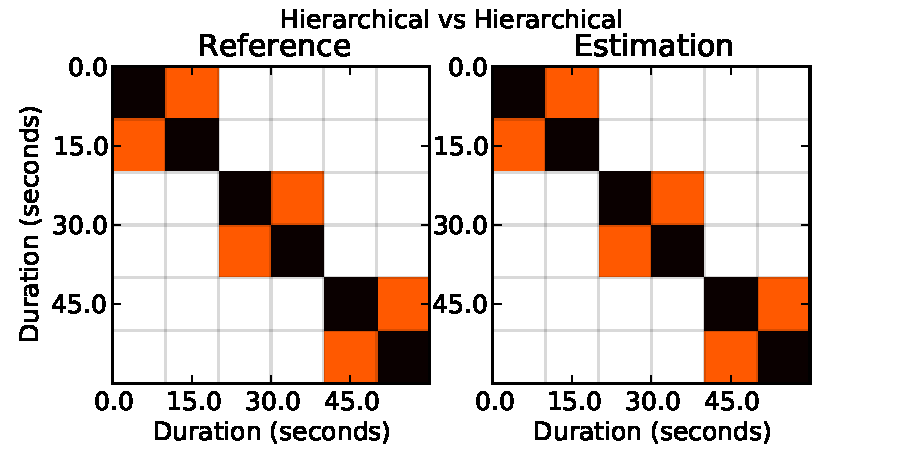
\includegraphics[width=0.94\textwidth]{figs/hier-hier.pdf}
%   \end{subfigure}%
%   \\
%   \begin{minipage}{0.5\textwidth}
%     \centering
%     \vspace{10pt}
%     \begin{tabular}{|c|c|c|}
%       \hline
%       $w$       & $\shag_u$    & $\shag_o$      \\
%       \hline
%       any       & 100       & 100      \\     
%       \hline
%     \end{tabular}
%   \end{minipage}
%   \caption{Hierarchical vs same hierarchical boundaries (top) and scores (bottom)}
%   \label{fig:hier-hier}
% \end{figure}

In \Cref{fig:hier-hiercomp}, the boundaries (top) and the results (bottom) of two different hierarchical segmentations are shown.
In this case, the estimated boundaries contain a third additional layer covering the first two large segments of its second layer.
Note that the lowest two layers of the estimation are exactly the same as the two layers of the reference.
The scores with a small window of 3 or less seconds show a perfect agreement for both $T$-measures grades.
However, as $w$ increases, we see how the over-segmentation grade $\shag_o$ decreases as expected, since the estimation has found an additional segment.
% (even if this new segment creates a new layer it still oversegments).
The under-segmentation grades remain at 100\% with any window length, as expected.


\begin{figure}[t]
  \centering
  \begin{subfigure}{0.5\textwidth}
    \centering
    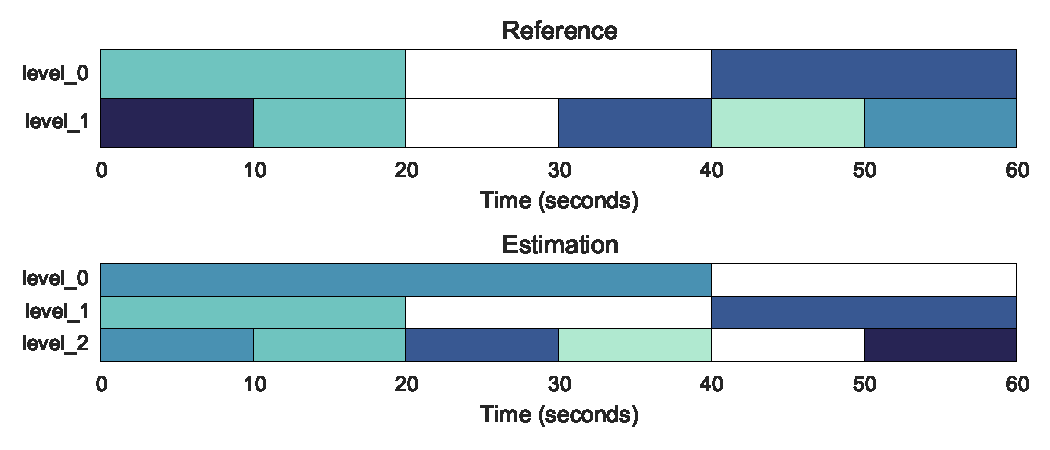
\includegraphics[width=0.94\textwidth]{figs/hier-hiercomp.pdf}
  \end{subfigure}%
  \\
  \begin{minipage}{0.5\textwidth}
    \centering
    \vspace{10pt}
    \begin{tabular}{|c|c|c|}
      \hline
      $w$       & $\shag_u$       & $\shag_o$      \\
      \hline
      0.5       & 100       & 100      \\     
      3         & 100       & 100      \\
      15        & 100       & 99.13    \\
      30        & 100       & 88.75    \\
      $\infty$  & 100       & 79.41    \\
      \hline
    \end{tabular}
  \end{minipage}
  \caption{2-layer vs. 3-layer hierarchical boundaries (top) and $T$-measures scores (bottom).}
  \label{fig:hier-hiercomp}
\end{figure}


\subsection{Real-world examples}
Finally, we examine the behavior of $T$-measures on real data, using two types of examples.
First, \Cref{fig:SALAMI-SALAMI} illustrates $T$-measures scores when comparing two manually-constructed hierarchical annotations on a track from the SALAMI dataset (making use of the large and small scale levels of segmentation).
While the two annotators tend to agree at the small scale, they differ at the large scale, and tend to group small-scale components in a slightly different manner from each-other.
This is reflected in the under- and over-segmentation scores: the former skews low, because the reference's large-scale annotations are coarser than those of the estimate, while the latter remains high because both tend to agree at the small scale.

\begin{figure}[t]
  \centering
  \begin{subfigure}{0.5\textwidth}
    \centering
    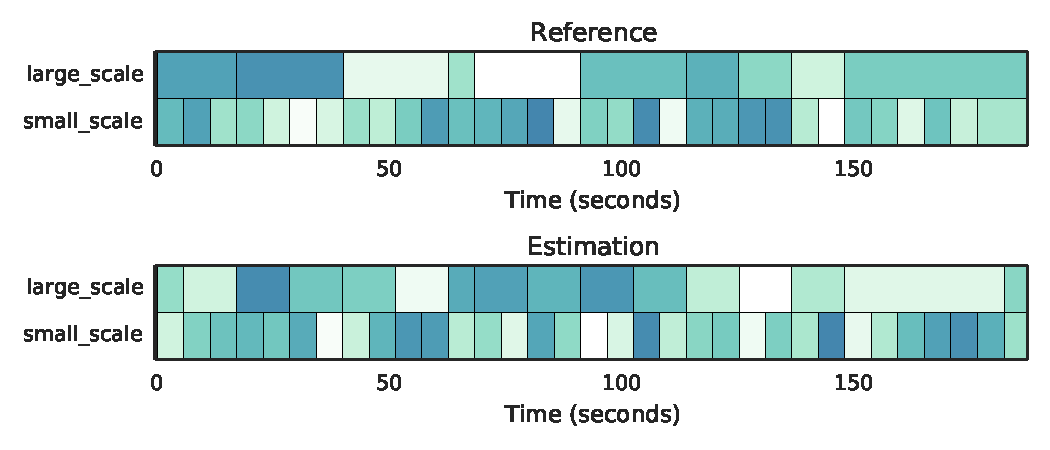
\includegraphics[width=0.99\textwidth]{figs/SALAMI-SALAMI.pdf}
  \end{subfigure}%
  \\
  \begin{minipage}{0.5\textwidth}
    \centering
    \vspace{10pt}
    \begin{tabular}{|c|c|c|}
      \hline
      $w$       & $\shag_u$       & $\shag_o$      \\
      \hline
      0.5       & 81.12       & 78.64      \\     
      3         & 96.08       & 93.02      \\
      15        & 80.37       & 83.79    \\
      30        & 70.53       & 89.01    \\
      $\infty$  & 67.50       & 97.51    \\
      \hline
    \end{tabular}
  \end{minipage}
  \caption{Hierarchical annotations for SALAMI track \#636 from the two different human annotators. Top: boundaries and frame-level segment agreement; bottom: $T$-measures scores.}
  \label{fig:SALAMI-SALAMI}
\end{figure}

% SALAMI 636 annotator 1 vs OLDA\cite{McFee2014}  output \ref{fig:SALAMI-OLDA}.
Finally, in the last example, we illustrate a comparison between a hierarchical estimation against a hierarchical reference, using the same SALAMI track.
The hierarchical estimation was produced by the agglomerative clustering method of McFee and Ellis~\cite{McFee2014}.
Note that the estimate produces many more layers than the reference, and the nesting structure is quite different.
In particular, the reference provides two levels of segmentation (large and small), while the estimate tends to mostly produce large segments, with more detailed nesting structure at even higher levels.

\begin{figure}[t]
  \centering
  \begin{subfigure}{0.5\textwidth}
    \centering
    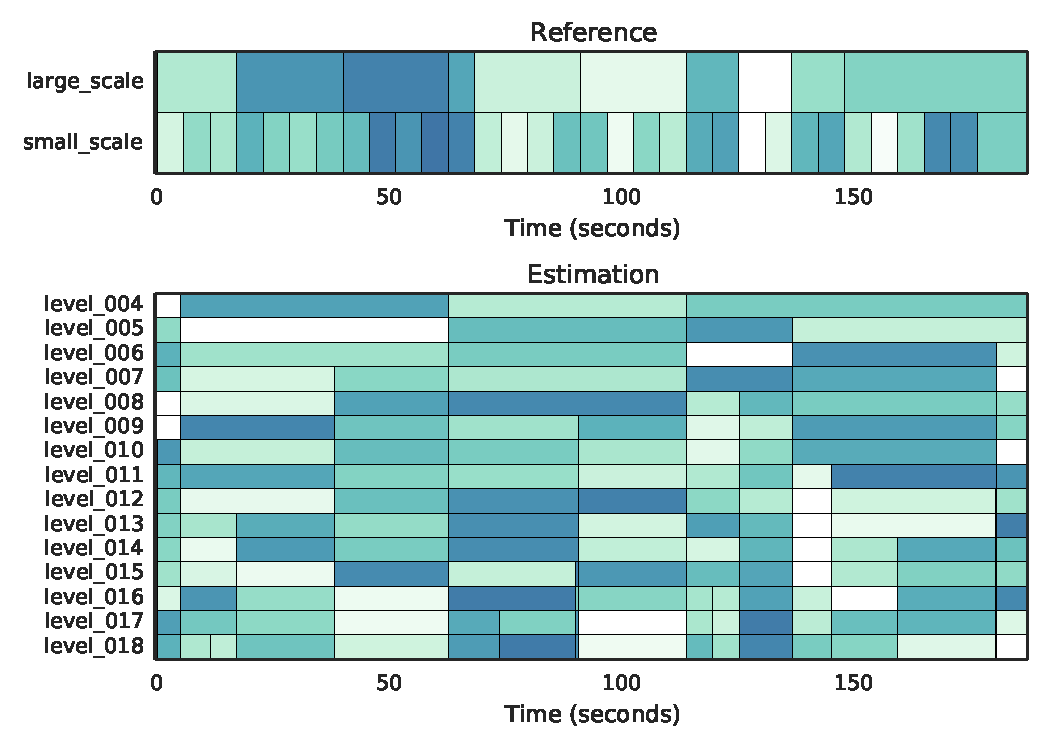
\includegraphics[width=0.94\textwidth]{figs/SALAMI-OLDA.pdf}
  \end{subfigure}%
  \\
  \begin{minipage}{0.5\textwidth}
    \centering
    \vspace{10pt}
    \begin{tabular}{|c|c|c|}
      \hline
      $w$       & $\shag_u$       & $\shag_o$      \\
      \hline
      0.5       & 27.72       & 54.54      \\     
      3         & 33.97       & 71.80      \\
      15        & 66.25       & 70.21    \\
      30        & 79.87       & 58.09    \\
      $\infty$  & 92.73       & 41.99    \\
      \hline
    \end{tabular}
  \end{minipage}
  \caption{Hierarchical annotation for SALAMI track \#636 vs.\ hierarchical boundary
  estimates~\cite{McFee2014} (top) and $T$-measures scores (bottom).}
  \label{fig:SALAMI-OLDA}
\end{figure}

%\section{Evaluating Automatic Algorithm}

%Olda\cite{McFee2014} with SALAMI.


\section{Conclusions}\label{sec:conclusions}

In this paper, we proposed a method to evaluate hierarchically structured boundary annotations. 
The proposed method facilitates simultaneous evaluation across multiple levels of detail simultaneously, and provides a holistic measure of how well a set of estimated structural boundaries matches a hierarchical reference. 
In the future, we plan to extend this general idea to other structural annotation problems, such as segment label agreement.

\bibliography{refs}

\end{document}
